\documentclass[a4paper,12pt]{article}
\usepackage{czech}
\usepackage[utf8]{inputenc}
\usepackage{a4wide}
\usepackage[dvipdfm]{graphicx}
\usepackage{graphics}
\usepackage{indentfirst}
\usepackage{fancyhdr}
\usepackage{setspace}
\usepackage{amsmath}
\usepackage{amssymb}
\usepackage{epsfig}

\usepackage[usenames]{color}
\begin{document}

\section{Úkol}
\begin{enumerate}
	\item Pro tři vodorovné trubice s různými poloměry kruhového průřezu, které jsou opatřeny manometry, 
	naměrte závislost objemového průtoku $Q_V$ na úbytku statického tlaku $\Delta p$ na vyšetřované délce trubice $l$ ve směru proudění.
	\item Sestrojte grafy závislosti $Q_V = Q_V(p)$. Do grafu zakreslete teoretický průběh této závislosti plynoucí z Poiseuillovy rovnice.
	\item Ze směrnice závislosti $Q_V = Q_V(p)$ v oblasti laminárního proudění urete poloměr trubice.
	\item Upravený poloměr dosaďte do vztahu pro výpočet $Re$ a $k$.
	\item Sestrojte graf závislosti $k=k(Re)$, kde $k$ je součinitel odporu trubice a $Re$ je Reynoldsovo číslo.
\end{enumerate}


\section{Teorie}
\noindent
Při proudění kapaliny trubicí rozlišujeme tři základní typy. Laminární, turbulentní a smíšené vzniklé střídáním předešlých dvou. 
K lepšímu určení toho, o který typ se zrova jedná se zavádí Reynoldosovo číslo definováno vztahem
\begin{eqnarray}
	Re=\frac{r \rho v_s}{\eta},
	\label{Re}
\end{eqnarray}
kde $r$ je poloměr trubice, $\rho$ hustota kapaliny, $v_s$ střední hodnota rychlosti proudění a $\eta$ dynamická viskozita kapaliny.
Při hodnotě tohoto čísla nižší než 2000 se přibližně jedná o laminární proudění. Od hodnoty 1000 se začínají objevovat trubulence.
Proto na intervalu od 1000 do 2000 vzniká proudění smíšené.

Pro laminární proudění platí Poissellova rovnice pro velikost průtoku trubicí
\begin{eqnarray}
	Q_V=\frac{\pi r^4}{8\eta l}\Delta p,
	\label{Poissell}
\end{eqnarray}
kde $r$ je poloměr trubice, $\eta$ dynamická viskozita a $\Delta p$ pokles tlaku v trubici na úseku délky $l$. V \cite{text} naleznete odvození 
vztahů potřebných pro úlohu. Nám postačí
\begin{eqnarray}
	Q_V=V/t \label{Q}\\
	\Delta p=h \rho g \label{p} \\
	Re=\frac{Q_V}{\pi r \eta}\rho \label{Re2} \\
	k=\frac{2\pi\Delta p r^5}{l\rho Q_V^2} \label{k}
\end{eqnarray}


\section{Výsledky měření}

\subsection{Podmínky}
\noindent
Teplota vody tekoucí trubicemi byla 22.5 $^{\circ}$C.

\subsection{Výpočty}
\noindent
Veškeré naměřené hodnoty byly statisticky vyhodnoceny dle \cite{chyba}. Tento zroj jsem také použil při stanovení chyb vypočítaných veličin. 
U odměrných válců jsem bral jako chybu měřidla polovinu nejmenšího dílku, chybu měření času jsem odhadl na 0.3 s a při stanovení výšky 
vodního sloupce v nanometru sjem počítal, až na vyjimky popsané níže s 1 mm.

Za hodnotu hustoty vody a dynamické viskozity jsem dosadil hodnoty z \cite{tabulky}
\begin{eqnarray}
	\rho=0.980 \mbox{kg}\cdot\mbox{m}^{-3}, \\
	\eta=1.002 \cdot 10^{-3} \mbox{Pa}\cdot\mbox{s}.
\end{eqnarray}

\subsection{Parametry trubicí}
\noindent
Poloměry trubic jsem měřil plastovým posuvným měřidlem, jejich délku metrem. Naměřené hodnoty naleznete v tabulce \ref{param}.
\begin{table}
$$
\begin{array}{|c|c|c|c|}
\hline
n&	r/\mbox{mm}&	r'/\mbox{mm}&	l/\mbox{cm}	\\ \hline
1&	1.8 \pm 0.1&	1.65 \pm 0.04&	20.1 \pm 0.1	\\ \hline
2&	1.6 \pm 0.1&	1.47 \pm 0.03&	25.1 \pm 0.1	\\ \hline
3&	1.1 \pm 0.1&	0.96 \pm 0.01&	25.0 \pm 0.1	\\ \hline
\end{array}
$$
\caption{Parametry trubic}
\label{param}
\end{table}

\subsection{Průtok trubicemi}
\noindent
Pro každou trubici jsem změřil objem $V$, který protekl trubicí za čas $t$ za výšky $h$ vodního sloupce v nanometru. Tyto hodnoty jsou v tabulkách \ref{T1}, \ref{T2} a \ref{T3}.


\begin{table}
$$
\begin{array}{|c|c|c|}
\hline
h/\mbox{cm}&	V/\mbox{ml}&	t/\mbox{s}	\\ \hline
1.5&	9.3 \pm 0.1&	17.0\pm 0.3\\ \hline
2.0&	24.0 \pm 0.3&	12.0\pm 0.3\\ \hline
2.5&	46.0 \pm 0.3&	16.8\pm 0.3\\ \hline
3.0&	94.0 \pm 1.0&	27.4\pm 0.3\\ \hline
3.5&	88.0 \pm 1.0&	21.4\pm 0.3\\ \hline
4.0&	88.0 \pm 1.0 &	18.6\pm 0.3\\ \hline
4.5&	80.0\pm 1.0&	15.0\pm 0.3\\ \hline
5.0&	90.0\pm 1.0&	15.4\pm 0.3\\ \hline
5.5&	88.0\pm 1.0&	14.4\pm 0.3\\ \hline
6.0&	88.0\pm 1.0&	13.0\pm 0.3\\ \hline
8.0 \pm 0.5&	82.0\pm 1.0&	10.8\pm 0.3\\ \hline
12.0 \pm 0.5&	90.0\pm 1.0&	11.2\pm 0.3\\ \hline
16.0&	92.0\pm 1.0&	9.8\pm 0.3\\ \hline
20.0&	88.0\pm 1.0&	8.2\pm 0.3\\ \hline
\end{array}
$$
\caption{Výsledky měření pro trubici 1.}
\label{T1}
\end{table}

\begin{table}
$$
\begin{array}{|c|c|c|}
\hline
h/\mbox{cm}&	V/\mbox{ml}&	t/\mbox{s}	\\ \hline
1.0&	8.9 \pm 0.1&	19.0\pm 0.3\\ \hline
2.0&	21.0 \pm 0.3&	16.4\pm 0.3\\ \hline
3.0&	24.0 \pm 0.3&	10.6\pm 0.3\\ \hline
4.0&	45.0 \pm 0.5&	14.6\pm 0.3\\ \hline
5.0&	49.0 \pm 0.5&	13.0\pm 0.3\\ \hline
6.0&	86.0 \pm 1.0 &	18.4\pm 0.3\\ \hline
7.0&	88.0 \pm 1.0&	18.2\pm 0.3\\ \hline
8.0&	86.0\pm 1.0&	16.0\pm 0.3\\ \hline
9.0&	88.0\pm 1.0&	15.0\pm 0.3\\ \hline
10.5 \pm 0.5&	84.0\pm 1.0&	13.8\pm 0.3\\ \hline
14.0 \pm 1.0&	90.0\pm 1.0&	13.0\pm 0.3\\ \hline
20.0 \pm 1.0&	88.0\pm 1.0&	11.8\pm 0.3\\ \hline
26.5&	90.0\pm 1.0&	10.6\pm 0.3\\ \hline
28.0&	94.0\pm 1.0&	11.0\pm 0.3\\ \hline
\end{array}
$$
\caption{Výsledky měření pro trubici 2.}
\label{T2}
\end{table}
\begin{table}
$$
\begin{array}{|c|c|c|}
\hline
h/\mbox{cm}&	V/\mbox{ml}&	t/\mbox{s}	\\ \hline
2&	9.4 \pm 0.1&	35.0\pm 0.3\\ \hline
4&	22.0 \pm 0.3&	39.6\pm 0.3\\ \hline
6&	21.5 \pm 0.3&	23.0\pm 0.3\\ \hline
8&	46.0 \pm 0.5&	32.4\pm 0.3\\ \hline
10&	47.0 \pm 0.5&	28.0\pm 0.3\\ \hline
12&	68.0 \pm 1.0 &	34.0\pm 0.3\\ \hline
14&	72.0\pm 1.0&	30.6\pm 0.3\\ \hline
16&	86.0\pm 1.0&	32.4\pm 0.3\\ \hline
18&	88.0\pm 1.0&	29.4\pm 0.3\\ \hline
20&	86.0\pm 1.0&	26.2\pm 0.3\\ \hline
22&	86.0\pm 1.0&	23.8\pm 0.3\\ \hline
24&	90.0\pm 1.0&	23.0\pm 0.3\\ \hline
\end{array}
$$
\caption{Výsledky měření pro trubici 3.}
\label{T3}
\end{table}



Z naměřených hodnot jsem vypočítal dle \ref{Q} a \ref{p} $Q_V$ a $\Delta p$ a zanesl je do grafu. Jeho hodnoty jsem v laminární časti 
za pomoci programu Gnuplot proložil přímkou a z její směrnice jsem stanovil skutečný poloměr trubic. Tyto hodnoty jsou pro možnost 
porovnání opět v tabulce \ref{param} označeny čárkou. Do grafu jsem ještě zanesl teoretické hodnoty $Q_V$ dle \ref{Poissell}. Výsledný 
graf naleznete pod obrázkem \ref{graf1}. 

\begin{figure}
\begin{center}
% GNUPLOT: LaTeX picture with Postscript
\begingroup
  \makeatletter
  \providecommand\color[2][]{%
    \GenericError{(gnuplot) \space\space\space\@spaces}{%
      Package color not loaded in conjunction with
      terminal option `colourtext'%
    }{See the gnuplot documentation for explanation.%
    }{Either use 'blacktext' in gnuplot or load the package
      color.sty in LaTeX.}%
    \renewcommand\color[2][]{}%
  }%
  \providecommand\includegraphics[2][]{%
    \GenericError{(gnuplot) \space\space\space\@spaces}{%
      Package graphicx or graphics not loaded%
    }{See the gnuplot documentation for explanation.%
    }{The gnuplot epslatex terminal needs graphicx.sty or graphics.sty.}%
    \renewcommand\includegraphics[2][]{}%
  }%
  \providecommand\rotatebox[2]{#2}%
  \@ifundefined{ifGPcolor}{%
    \newif\ifGPcolor
    \GPcolorfalse
  }{}%
  \@ifundefined{ifGPblacktext}{%
    \newif\ifGPblacktext
    \GPblacktexttrue
  }{}%
  % define a \g@addto@macro without @ in the name:
  \let\gplgaddtomacro\g@addto@macro
  % define empty templates for all commands taking text:
  \gdef\gplbacktext{}%
  \gdef\gplfronttext{}%
  \makeatother
  \ifGPblacktext
    % no textcolor at all
    \def\colorrgb#1{}%
    \def\colorgray#1{}%
  \else
    % gray or color?
    \ifGPcolor
      \def\colorrgb#1{\color[rgb]{#1}}%
      \def\colorgray#1{\color[gray]{#1}}%
      \expandafter\def\csname LTw\endcsname{\color{white}}%
      \expandafter\def\csname LTb\endcsname{\color{black}}%
      \expandafter\def\csname LTa\endcsname{\color{black}}%
      \expandafter\def\csname LT0\endcsname{\color[rgb]{1,0,0}}%
      \expandafter\def\csname LT1\endcsname{\color[rgb]{0,1,0}}%
      \expandafter\def\csname LT2\endcsname{\color[rgb]{0,0,1}}%
      \expandafter\def\csname LT3\endcsname{\color[rgb]{1,0,1}}%
      \expandafter\def\csname LT4\endcsname{\color[rgb]{0,1,1}}%
      \expandafter\def\csname LT5\endcsname{\color[rgb]{1,1,0}}%
      \expandafter\def\csname LT6\endcsname{\color[rgb]{0,0,0}}%
      \expandafter\def\csname LT7\endcsname{\color[rgb]{1,0.3,0}}%
      \expandafter\def\csname LT8\endcsname{\color[rgb]{0.5,0.5,0.5}}%
    \else
      % gray
      \def\colorrgb#1{\color{black}}%
      \def\colorgray#1{\color[gray]{#1}}%
      \expandafter\def\csname LTw\endcsname{\color{white}}%
      \expandafter\def\csname LTb\endcsname{\color{black}}%
      \expandafter\def\csname LTa\endcsname{\color{black}}%
      \expandafter\def\csname LT0\endcsname{\color{black}}%
      \expandafter\def\csname LT1\endcsname{\color{black}}%
      \expandafter\def\csname LT2\endcsname{\color{black}}%
      \expandafter\def\csname LT3\endcsname{\color{black}}%
      \expandafter\def\csname LT4\endcsname{\color{black}}%
      \expandafter\def\csname LT5\endcsname{\color{black}}%
      \expandafter\def\csname LT6\endcsname{\color{black}}%
      \expandafter\def\csname LT7\endcsname{\color{black}}%
      \expandafter\def\csname LT8\endcsname{\color{black}}%
    \fi
  \fi
  \setlength{\unitlength}{0.0500bp}%
  \begin{picture}(11904.00,8502.00)%
    \gplgaddtomacro\gplbacktext{%
      \csname LTb\endcsname%
      \put(1078,704){\makebox(0,0)[r]{\strut{} 0}}%
      \put(1078,2488){\makebox(0,0)[r]{\strut{} 0,5}}%
      \put(1078,4273){\makebox(0,0)[r]{\strut{} 1}}%
      \put(1078,6057){\makebox(0,0)[r]{\strut{} 1,5}}%
      \put(1078,7841){\makebox(0,0)[r]{\strut{} 2}}%
      \put(1210,484){\makebox(0,0){\strut{} 0}}%
      \put(3203,484){\makebox(0,0){\strut{} 5}}%
      \put(5196,484){\makebox(0,0){\strut{} 10}}%
      \put(7189,484){\makebox(0,0){\strut{} 15}}%
      \put(9182,484){\makebox(0,0){\strut{} 20}}%
      \put(11174,484){\makebox(0,0){\strut{} 25}}%
      \put(308,4272){\rotatebox{-270}{\makebox(0,0){\strut{}\rotatebox{-90}{$\frac{U}{\mathrm{V}}$}}}}%
      \put(6391,154){\makebox(0,0){\strut{}$\frac{I}{\mathrm{mA}}$}}%
      \put(6391,8171){\makebox(0,0){\strut{}Graf 1: Z\'avislost nap\v{e}t\'i na proudu}}%
    }%
    \gplgaddtomacro\gplfronttext{%
      \csname LTb\endcsname%
      \put(10586,1482){\makebox(0,0)[r]{\strut{}$U(I)$}}%
      \csname LTb\endcsname%
      \put(10586,1196){\makebox(0,0)[r]{\strut{}$U(I)$}}%
      \csname LTb\endcsname%
      \put(10586,910){\makebox(0,0)[r]{\strut{}$T_m$}}%
    }%
    \gplbacktext
    \put(0,0){\includegraphics{graf1}}%
    \gplfronttext
  \end{picture}%
\endgroup

\end{center}
\caption{Graf závislosti $Q_V$ na $\Delta p$}
\label{graf1}
\end{figure}

\subsection{Závislot odporu trubice na Reynoldově čísle}
\noindent
Dle vztahů \ref{Re2}, \ref{k}, dopočtených poloměrů a naměřených hodnot sestrojil graf závislost $k$ na $Re$. Jedná 
se o obrázek \ref{graf2}. Dále jsem zanesl teoretickou závislost pro laminární a turbuletní proudění zmíněnou v \cite{text}.

\begin{figure}
\begin{center}
% GNUPLOT: LaTeX picture with Postscript
\begingroup
  \makeatletter
  \providecommand\color[2][]{%
    \GenericError{(gnuplot) \space\space\space\@spaces}{%
      Package color not loaded in conjunction with
      terminal option `colourtext'%
    }{See the gnuplot documentation for explanation.%
    }{Either use 'blacktext' in gnuplot or load the package
      color.sty in LaTeX.}%
    \renewcommand\color[2][]{}%
  }%
  \providecommand\includegraphics[2][]{%
    \GenericError{(gnuplot) \space\space\space\@spaces}{%
      Package graphicx or graphics not loaded%
    }{See the gnuplot documentation for explanation.%
    }{The gnuplot epslatex terminal needs graphicx.sty or graphics.sty.}%
    \renewcommand\includegraphics[2][]{}%
  }%
  \providecommand\rotatebox[2]{#2}%
  \@ifundefined{ifGPcolor}{%
    \newif\ifGPcolor
    \GPcolorfalse
  }{}%
  \@ifundefined{ifGPblacktext}{%
    \newif\ifGPblacktext
    \GPblacktexttrue
  }{}%
  % define a \g@addto@macro without @ in the name:
  \let\gplgaddtomacro\g@addto@macro
  % define empty templates for all commands taking text:
  \gdef\gplbacktext{}%
  \gdef\gplfronttext{}%
  \makeatother
  \ifGPblacktext
    % no textcolor at all
    \def\colorrgb#1{}%
    \def\colorgray#1{}%
  \else
    % gray or color?
    \ifGPcolor
      \def\colorrgb#1{\color[rgb]{#1}}%
      \def\colorgray#1{\color[gray]{#1}}%
      \expandafter\def\csname LTw\endcsname{\color{white}}%
      \expandafter\def\csname LTb\endcsname{\color{black}}%
      \expandafter\def\csname LTa\endcsname{\color{black}}%
      \expandafter\def\csname LT0\endcsname{\color[rgb]{1,0,0}}%
      \expandafter\def\csname LT1\endcsname{\color[rgb]{0,1,0}}%
      \expandafter\def\csname LT2\endcsname{\color[rgb]{0,0,1}}%
      \expandafter\def\csname LT3\endcsname{\color[rgb]{1,0,1}}%
      \expandafter\def\csname LT4\endcsname{\color[rgb]{0,1,1}}%
      \expandafter\def\csname LT5\endcsname{\color[rgb]{1,1,0}}%
      \expandafter\def\csname LT6\endcsname{\color[rgb]{0,0,0}}%
      \expandafter\def\csname LT7\endcsname{\color[rgb]{1,0.3,0}}%
      \expandafter\def\csname LT8\endcsname{\color[rgb]{0.5,0.5,0.5}}%
    \else
      % gray
      \def\colorrgb#1{\color{black}}%
      \def\colorgray#1{\color[gray]{#1}}%
      \expandafter\def\csname LTw\endcsname{\color{white}}%
      \expandafter\def\csname LTb\endcsname{\color{black}}%
      \expandafter\def\csname LTa\endcsname{\color{black}}%
      \expandafter\def\csname LT0\endcsname{\color{black}}%
      \expandafter\def\csname LT1\endcsname{\color{black}}%
      \expandafter\def\csname LT2\endcsname{\color{black}}%
      \expandafter\def\csname LT3\endcsname{\color{black}}%
      \expandafter\def\csname LT4\endcsname{\color{black}}%
      \expandafter\def\csname LT5\endcsname{\color{black}}%
      \expandafter\def\csname LT6\endcsname{\color{black}}%
      \expandafter\def\csname LT7\endcsname{\color{black}}%
      \expandafter\def\csname LT8\endcsname{\color{black}}%
    \fi
  \fi
  \setlength{\unitlength}{0.0500bp}%
  \begin{picture}(7200.00,5040.00)%
    \gplgaddtomacro\gplbacktext{%
      \csname LTb\endcsname%
      \put(1210,704){\makebox(0,0)[r]{\strut{} 0}}%
      \put(1210,1722){\makebox(0,0)[r]{\strut{} 0.05}}%
      \put(1210,2740){\makebox(0,0)[r]{\strut{} 0.1}}%
      \put(1210,3757){\makebox(0,0)[r]{\strut{} 0.15}}%
      \put(1210,4775){\makebox(0,0)[r]{\strut{} 0.2}}%
      \put(1342,484){\makebox(0,0){\strut{} 0}}%
      \put(2447,484){\makebox(0,0){\strut{} 500}}%
      \put(3553,484){\makebox(0,0){\strut{} 1000}}%
      \put(4658,484){\makebox(0,0){\strut{} 1500}}%
      \put(5764,484){\makebox(0,0){\strut{} 2000}}%
      \put(6869,484){\makebox(0,0){\strut{} 2500}}%
      \put(308,2739){\rotatebox{-270}{\makebox(0,0){\strut{}$k$}}}%
      \put(4105,154){\makebox(0,0){\strut{}$Re$}}%
    }%
    \gplgaddtomacro\gplfronttext{%
      \csname LTb\endcsname%
      \put(5882,4602){\makebox(0,0)[r]{\strut{}Trubice 1}}%
      \csname LTb\endcsname%
      \put(5882,4382){\makebox(0,0)[r]{\strut{}Trubice 2}}%
      \csname LTb\endcsname%
      \put(5882,4162){\makebox(0,0)[r]{\strut{}Trubice 3}}%
      \csname LTb\endcsname%
      \put(5882,3942){\makebox(0,0)[r]{\strut{}16/$Re$}}%
      \csname LTb\endcsname%
      \put(5882,3722){\makebox(0,0)[r]{\strut{}0.133/Re$^{1/4}$}}%
    }%
    \gplbacktext
    \put(0,0){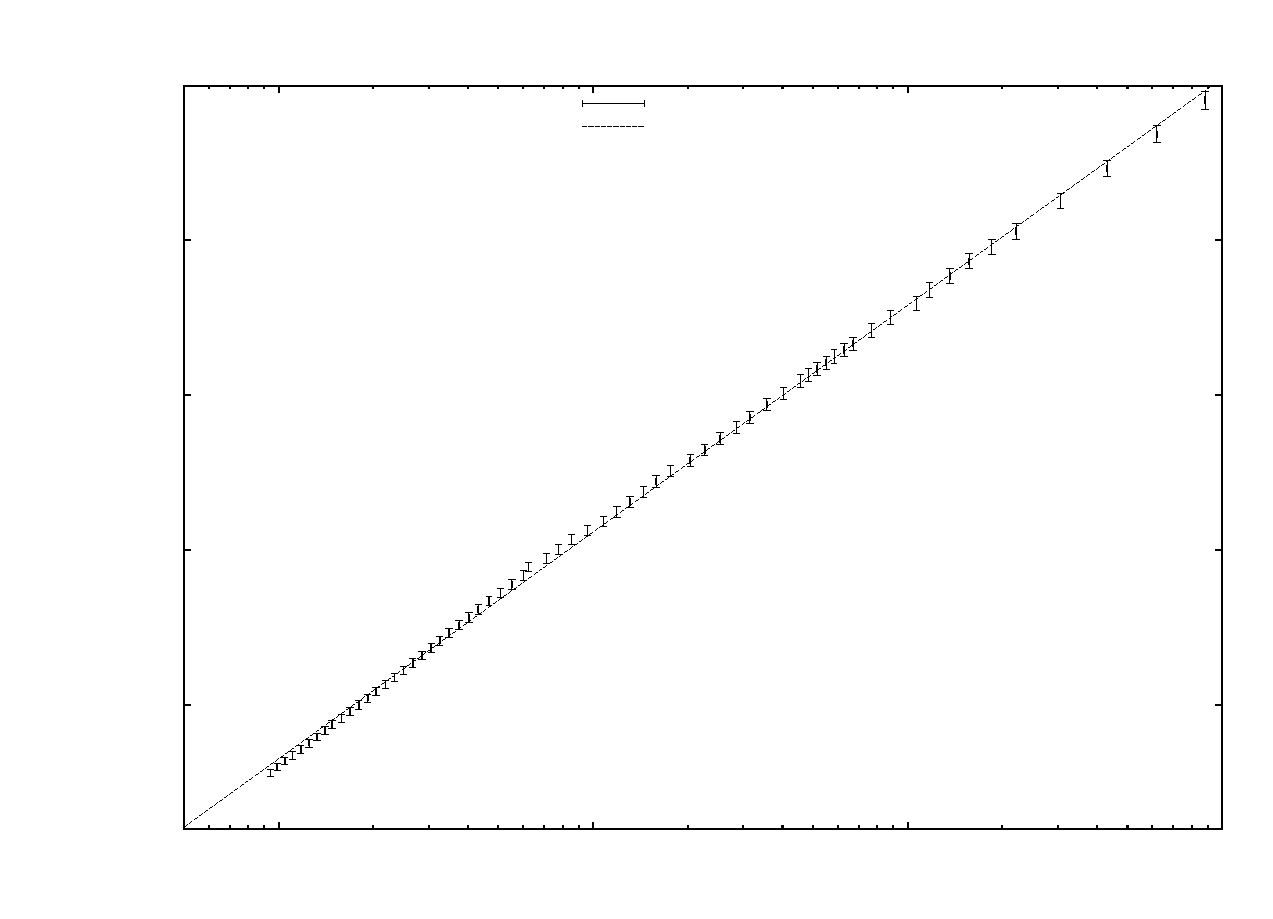
\includegraphics{graf2}}%
    \gplfronttext
  \end{picture}%
\endgroup

\end{center}
\caption{Graf závislosti $k$ na $Re$}
\label{graf2}
\end{figure}

\section{Diskuze}
\noindent
Mnou naměřené hodnoty v oblasti laminárního proudění dobře odpovídají teoretickým hodnotám daným Poissellovou rovnicí. Závíslost $k$ na $Re$ 
v oblasti proudění není, obzvláště u trubice 2, tak přesná.  V oblasti smíšeného proudění jsou hodnoty pouze orientační, protože vlivem 
častého střídání typu porudění nebylo možné přesně stanmovit $\Delta p$.

Menší nesnáze jsou měl s kouhoutkem korigujícím průtok hadicemi. Místy bylo nastavení přesného tlaku vcelku nesnadné a záleželo na tom, 
zda se zrovna člověk kohoutku dotýkal či nikoliv. Dále by nebylo šatné trochu zvýšit stojan s trubicemi, protože větší odměrné válce se při 
měření museli držet šikmo.

Díky velkému času a relativně velkému objemu vody při měření byla výsledná chyba malá, a proto nebylo třeba měření opakovat.

\section{Závěr}
Změřil jsem závislot objemového průtoku na úbytku tlaku ve třech trubicích. Tuto závislost jsem zanesl do grafu, který je označen jako 
obrázek \ref{graf1}.

Ze směrnice grafu $Q_V=Q_V(\Delta p)$ v oblasti laminárního proudění jsem stanovil skutečné poloměry trubic
\begin{eqnarray}
r'_1=(1.65\pm0.04)\mbox{mm} \\
r'_2=(1.47\pm0.03)\mbox{mm} \\
r'_2=(0.96\pm0.01)\mbox{mm} 
\end{eqnarray}

Dosazením skutečných poloměrů do rovnic \ref{Re} a \ref{k} jsem dopočetl $Re$ a $k$ a jejich závislost zanesl do grafu označeným obrázek \ref{graf2}.


\begin{thebibliography}{5}
        \bibitem{text} \textbf{Studijní text na praktikum I} \\http://physics.mff.cuni.cz/vyuka/zfp/txt\_103.pdf (26. 4. 2011)
        \bibitem{kvasnica} \emph{Prof. RNDr. Jozef Kvasnica, DrSc. a kolektiv}: \textbf{Mechanika}\\ Academia, Praha 1988
        \bibitem{chyba} \emph{J. Englich}: \textbf{Zpracování výsldků fyzikálních měření} \\ LS 1999/2000
       \bibitem{tabulky} \emph{Jiří Mikulčák a kolektiv}: \textbf{Matematické, fyzikální a chemické tabulky} \\ Prometheus, Praha 1988

\end{thebibliography}

\end{document}
